\begin{frame}{The \tHq lepditau channel}
%  \begin{columns}
%    \begin{column}{0.5\textwidth}
  \begin{itemize}
  \item Monte Carlo generators: Pythia8, Powheg
\end{itemize}
     \begin{figure}
        \centering
        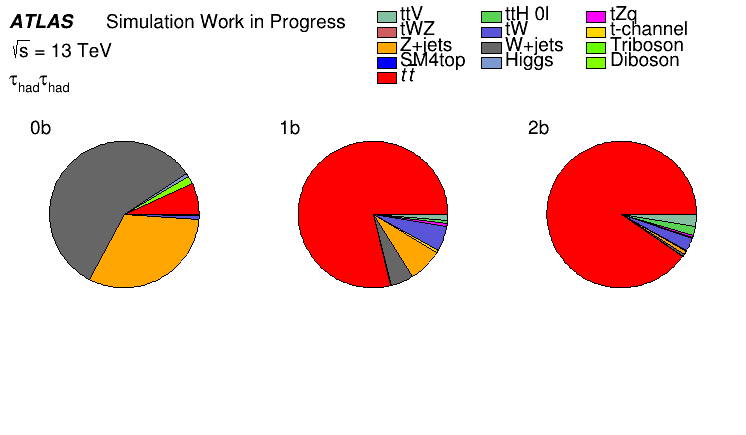
\includegraphics[width=0.95\textwidth]{PieChart_hadhad.png}
      \end{figure}
%    \end{column}
%    \begin{column}{0.5\textwidth}
%      \begin{itemize}
%        \item Relatively high branching ratio
%        \vspace{0.3cm}
%        \item Hadronically decaying taus are more difficult to select than leptonic ones
%     \end{itemize}
%    \end{column}
% \end{columns}

\end{frame}


\begin{frame}{\tHq lepditau channel selection}
  \begin{columns}
    \begin{column}{0.5\textwidth}
      \centering 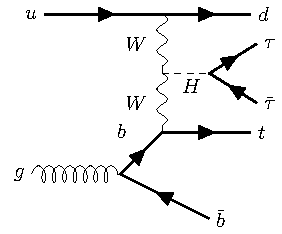
\includegraphics[width=\textwidth]{tHq_tautau}\\
      %\includegraphics[width=0.45\textwidth]{/cephfs/user/s6chkirf/feynman_diagrams/tHq_WW}
      %\includegraphics[width=0.45\textwidth]{/cephfs/user/s6chkirf/feynman_diagrams/tHq_ZZ}
    \end{column}
    \begin{column}{0.5\textwidth}
      \begin{block}{Coarse selection}
         \begin{itemize}
           \item Number of jets: 2
           \item Number of b-jets: 1
           \item number of leptons: \bf{$1e / \mu$}
           \item number of taus: 2 hadronic taus
           \item $E_{\text{T,miss}}$: no cut (to \SI{800}{GeV})
         \end{itemize}
      \end{block}
    \end{column}
  \end{columns}
\end{frame}
  
